\documentclass[a4paper,12pt]{article}
%For images
\usepackage{graphicx}
 
\addtolength{\oddsidemargin}{-.875in}
\addtolength{\evensidemargin}{-.875in}
\addtolength{\textwidth}{1.75in}
 
\addtolength{\topmargin}{-.875in}
\addtolength{\textheight}{1.75in}
 
\begin{document}
\begin{enumerate}
    \item \begin{enumerate}
        \item Med produktregeln blir derivatan
        $$x'cos(x)+x(cos(x))'=cos(x)-xsin(x)$$

        \item Med produktregeln blir derivatan
        $$\frac{e^x}{x}-\frac{e^x}{x^2}$$
    \end{enumerate}

    \item \begin{enumerate}
        \item Derivatan är 

        \item $$y'(x)=-\frac{4}{x^2}+\frac{1}{x}$$
        Så 
        $$y'(2)=-\frac{4}{4}+\frac{1}{2}=-0.5$$

        Vilket kan verifieras med en bild

        \begin{center}
            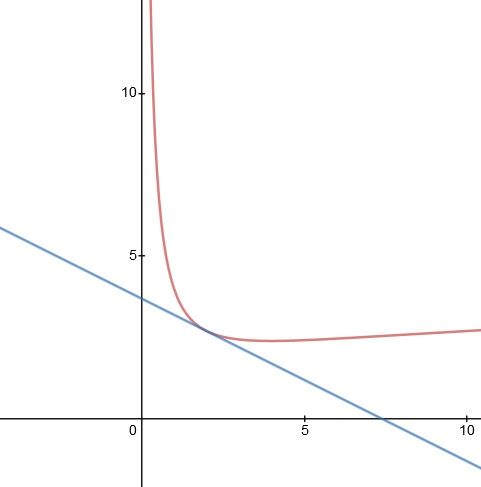
\includegraphics[scale=0.5]{Figur 1.jpg}
        \end{center}
    \end{enumerate}

    \item
    Derivatan blir
    $$\frac{10}{x}-2x+8$$

    Som illustreras som röd medans den svarta är orginalekvationen.
    
    \begin{center}
        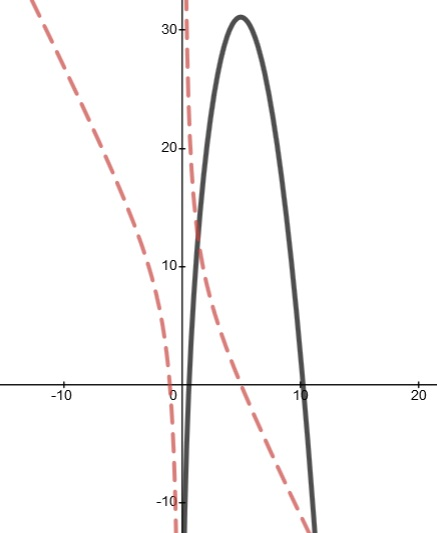
\includegraphics[scale=0.6]{Figur 2.jpg}
    \end{center}
    
    Extrempunkterna hamnar där derivatan är noll
    $$\frac{10}{x}-2x+8=0$$
    Skriver om den till en andragradsekvation
    $$10-2x^2=-8x\Rightarrow x^2-4x-5=0\Rightarrow (x-5)(x+1)=0$$
    Extrempunkterna sker då vid 5 och -1.
    Man kan se vid dom olika omskrivningarna av derivatan
    så behåller möter dom fortfarande varandra på x-axeln.
    Att manipulera polynomer som man sätter lika med noll är samma
    som att transformera kurvan i det tvådimensionella planet som behåller
    punkten.

    \begin{center}
        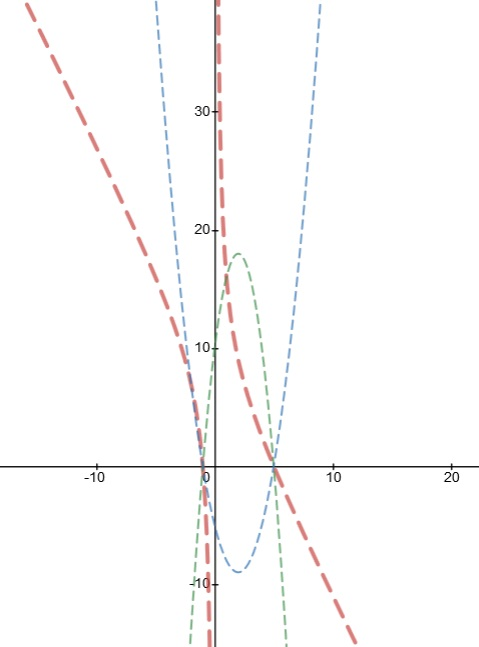
\includegraphics[scale=0.6]{Figur 3.jpg}
    \end{center}

    Men eftersom att den orginella ekvationen inehåller
    $10ln(x)$ så är den odefinierad för reella variabler.
    Då lär jag svara att det finns en extrempunkt vid x=5

    Tar man andraderivatan $-\frac{10}{x^2}-2$ vid x=5 får man att 
    andraderivatan är negativ, vilket innebär att det är en maximipunkt.   
    Detta kan man se i figur 2. 

    \item 
    Ekvationen för en tangent vid punkt $x_0$ är
    $f'(x_0)x+f(x_0)-f'(x_0)x_0$.
    
    Eftersom att $x_0=0$ så simplifieras den till
    $f'(0)x+f(0)$.

    $f(0)=4\sin(2\cdot 0)+\cos(0)=1$

    $f'(x)=8cos(2x)-sin(x)$
    
    $f'(0)=8cos(2\cdot 0)-sin(0)=8$

    Så då blir tangenten och svaret på frågan följande:
    $f'(0)x+f(0)=8x+1$

    I figuren nedan är tangenten blå, derivatan lila 
    och den orginella ekvationen är röd. Observera att 
    y och x axlarna inte har samma skala.

    \begin{center}    
        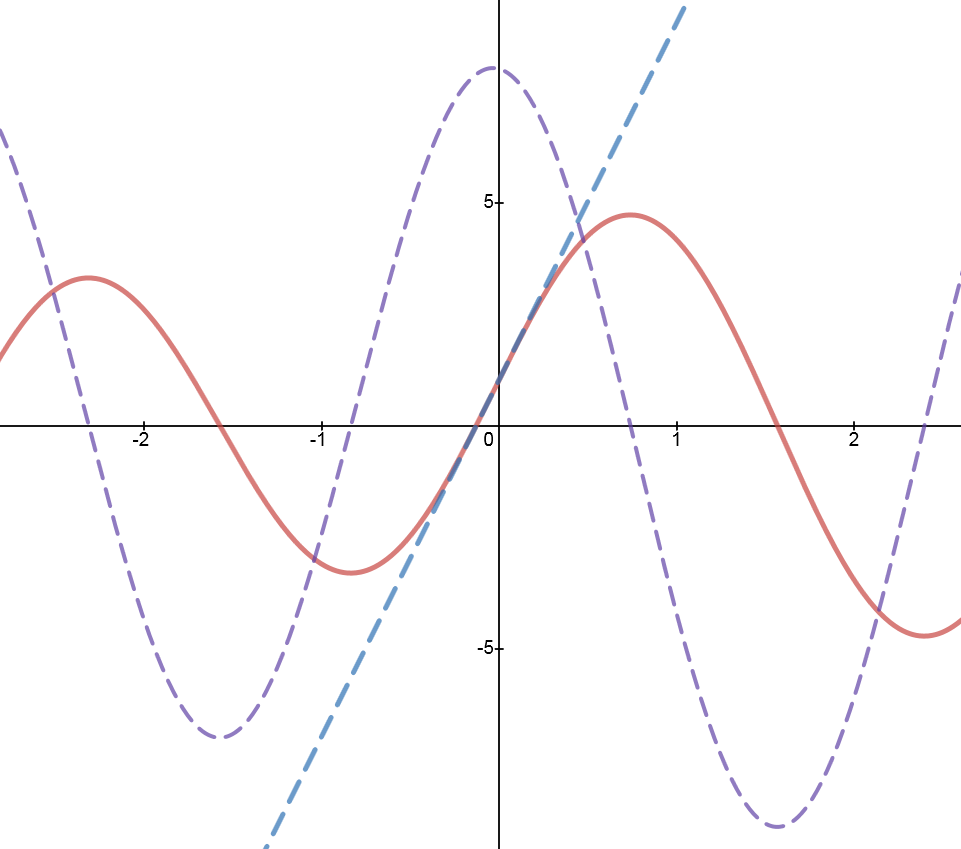
\includegraphics[scale=0.5]{Figur4.png}
    \end{center}

    \item Asymptoterna är ställen i funktionen där man delar på noll.
    Vid $$y=\frac{2}{x-3}+4$$ är det självklart att 3 är en assymptot.
    På y-axeln sker det också en asymptot. 4:an i ekvationen
    får en att tänka sig att det sker då (se figur nedan) eftersom
    att 4 transformerar hela grafen upp med 4. Men för att göra detta 
    rigoröst lösar man ut x
    $$y-4=\frac{2}{x-3}\Rightarrow x-3=\frac{2}{y-4}\Rightarrow x=\frac{2}{y-4}+3 $$

    Detta visar att y=4 är den andra asymptoten.
    
    \begin{center}
        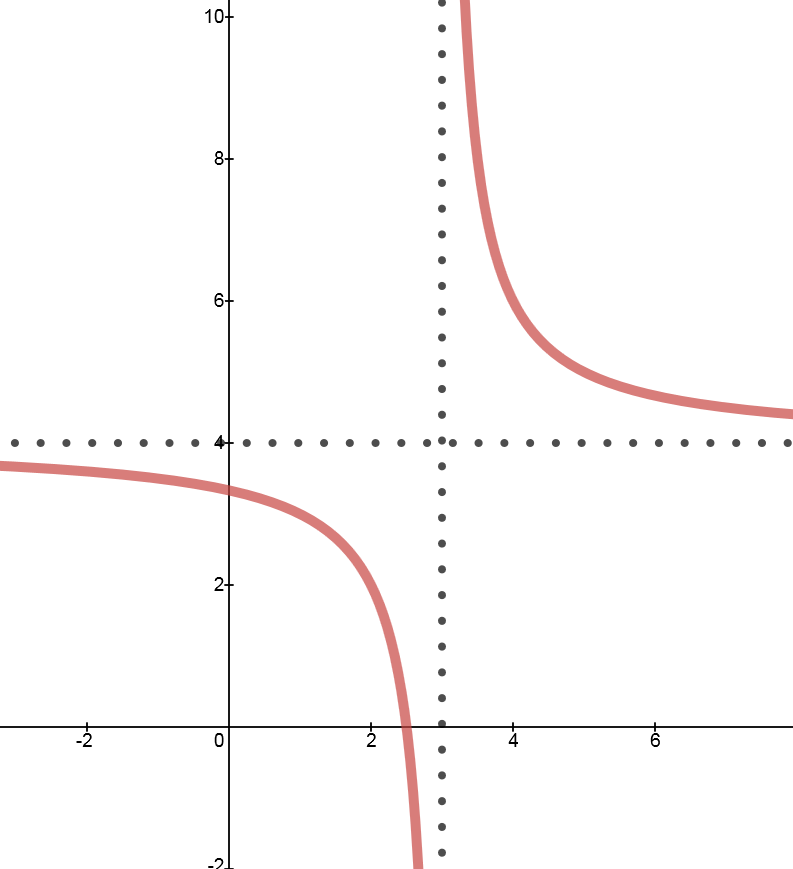
\includegraphics[scale=0.5]{Figur5.png}
    \end{center}

    \item 
    I uppgiften får vi reda på två sanningar. Med följande variabler

    \begin{center}
        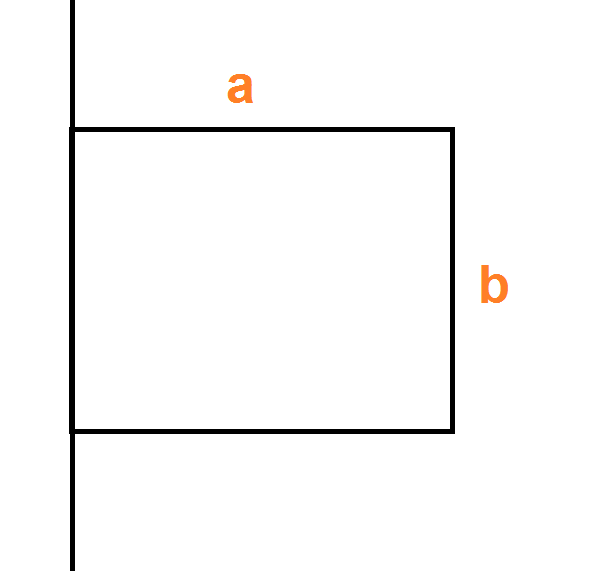
\includegraphics[scale=0.4]{Figur 6.png}
    \end{center}
    
    Får vi ut att Arean $A=ab$ och omkretsen $O=50=2a+b$
    Omkretsekvationen kan skrivas om som $b=50-2a$ och sedan 
    sättas in i den första vilket bildar $A=a(50-2a)=50a-2a^2$.

    Maxpunkten blir då där derivatan av funktionen är noll.
    $50-4a=0\Rightarrow a=12.5$ meter.

    Så när a är 12.5 meter blir det optimal area, och följande 
    ekvationen kring omkretsen måste b ha längden $50-2\cdot 12.5=25$ meter.

    \item 
    Med produktregeln blir derivatan
    $(x^2)'2^x+x^2(2^x)'=2x\cdot 2^x + x^2\cdot 2^x\cdot ln(2)$

    Och dom blir noll när 
    $$0=2x\cdot 2^x + x^2\cdot 2^x\cdot ln(2)$$
    $$-x^2\cdot 2^x\cdot ln(2)=2x\cdot 2^x $$
    $$-x^2\cdot ln(2)=2x$$
    $$-x\cdot ln(2)=2$$
    $$x=-\frac{2}{ln(2)}$$
    
    Men eftersom det är en andragradsekvation så finns det ett till 
    svar som man enkelt kan se är $x=0$.
    
    Ett till svar (kanske?) är "minus oändlighet", men man kan inte bara sätta
    in det utan man lär använda sig av gränsvärden
    $$\lim_{x\rightarrow -\infty}2x\cdot 2^x + x^2\cdot 2^x\cdot ln(2)
    =\lim_{x\rightarrow -\infty}2^{x}
    =\lim_{x\rightarrow \infty}2^{-x}
    =\lim_{x\rightarrow \infty}\frac{1}{2^x}
    =0$$

    \item I uppgiften får vi differentialekvationen $\frac{dr}{dt}=3$ 
    där r är radien och t är tid. Vi vet även att Arean av en cirkel är 
    $A=\pi r^2$. Vi löser ekvationen 
    $dr=3dt\Rightarrow \int dr =\int 3dt
    \Rightarrow r=3t+c$.
    Men vi kan anta att konstanten $c=0$ om början av olyckan var vid en punkt.
    
    Sedan stoppas den in i Area ekvationen $A=\pi (3t)^2=\pi 9t^2$. 
    Frågan är hur fort arean ökar, så då deriveras ekvationen med respekt av tid
    och man får $\frac{dA}{dt}=\pi 18t$. Vid tid $t=5$ så ökar arean med $\pi 18\cdot 5=90\pi \approx 282 m^2/s$
    
    FEL SVAARARARAARAR DEN ÄR OMÖJLIGT SÅ SNABBT VÄXANDE

    \item 
    Jag börjar med att skriva om ekvationen så den 
    blir enklare att derivera.
    $$f(x):=\frac{x^2+3}{x-1}$$
    $$(x^2+3)(x-1)^{-1}$$
    
    Nu deriveras det. Med produktregeln blir det 
    $$f'(x)=(x-1)^{-1}(x^2+3)'+((x-1)^{-1})'(x^2+3)$$
    
    Jag börjar med att derivera $(x-1)^{-1}$.
    Låt $u=x-1$ och $y=\frac{1}{u}$.
    Med Leibniz notering 
    $$\frac{dy}{dx}=\frac{dy}{du}\cdot \frac{du}{dx}
    =-\frac{3}{u^2}\cdot 1=-\frac{1}{(x-1)^2}$$
    
    Sammtidigt blir derivatan för $x^2+3=2x$
    Då blir det 
    $$f'(x)=(x-1)^{-1}2x-\frac{1}{(x-1)^2}(x^2+3)$$
    $$=\frac{2x}{x-1}-\frac{x^2+3}{(x-1)^2}$$
    
    Extrempunkterna där derivatan är noll och
    andraderivatan är negativ är där 
    maxpunkter finns. 
    
    $$0=\frac{2x}{x-1}-\frac{x^2+3}{(x-1)^2}$$
    $$\frac{x^2+3}{(x-1)^2}=\frac{2x}{x-1}$$
    $$\frac{x^2+3}{x-1}={2x}$$
    $$x^2+3=2x(x-1)$$
    $$x^2+3=2x^2-2x$$
    $$0=x^2-2x-3$$
    $$0=(x-3)(x+1)$$
    Extrempunkter sker vid 3 och -1. Med hjälp av andraderivatan
    kan man ta reda på vilka som är min, max eller terraspunkt.
    
    $$f''(x)=(\frac{2x}{x-1})'-(\frac{x^2+3}{(x-1)^2})'$$
    
    Där 
    $$(2x(x-1)^{-1})'=\frac{2}{x-1}-\frac{2x}{(x-1)^2}$$
    
    Och
    $$(\frac{x^2+3}{(x-1)^2})'=$$

\end{enumerate}
\end{document}